% ============================================================
% §2.4  Existing approaches: fixed representations and representational change
% ============================================================

\section{Related Work in Learning and Planning Under Novelty}
\label{sec:what_field_does}
\label{sec:capabilities_and_gaps}

Measured against the requirements identified in \cref{sec:what_is_required}, existing methods fall into a useful pattern.
The most mature approaches support detection, re-estimation, robustness, replanning, or rapid adaptation, but often do so while keeping the agent's representational vocabulary fixed.
A smaller body of work extends the agent's representation in response to failure, but usually pays for that capacity in speed, scope, or reliance on strong structure supplied in advance.
This section organizes existing work around that trade-off.
\Cref{fig:requirements_coverage} previews the resulting picture: each method family is measured against the four requirements from \cref{sec:what_is_required}, and the survey below follows the same organization.

% Requirements coverage matrix
\begin{figure}[t]
    \centering
    \resizebox{0.98\textwidth}{!}{%
    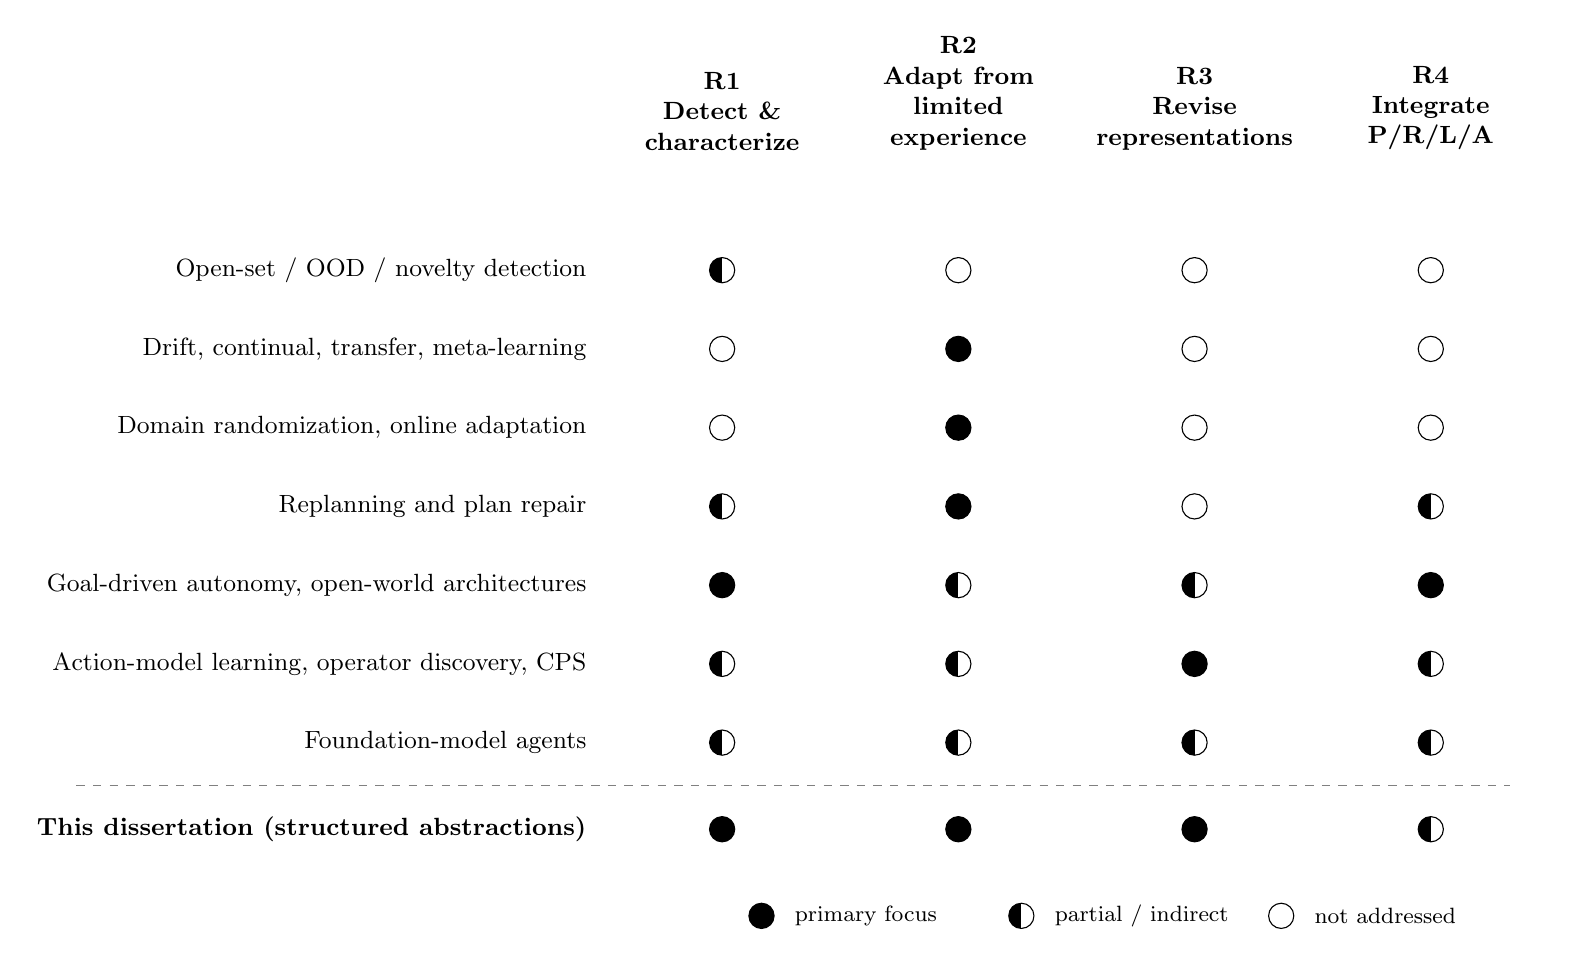
\begin{tikzpicture}[
        rowlabel/.style={anchor=east, align=right, font=\small},
        collabel/.style={anchor=south, align=center, font=\small\bfseries, text width=2.6cm},
        full/.style={circle, draw, fill=black, minimum size=0.32cm, inner sep=0pt},
        half/.style={circle, draw, minimum size=0.32cm, inner sep=0pt, path picture={\fill (path picture bounding box.south west) rectangle (path picture bounding box.north);}},
        none/.style={circle, draw, minimum size=0.32cm, inner sep=0pt},
    ]
    % Column x-positions
    \def\cA{0.0}  % R1 detect & characterize
    \def\cB{3.0}  % R2 adapt from limited experience
    \def\cC{6.0}  % R3 revise representations
    \def\cD{9.0}  % R4 integrate P/R/L/A

    % ===== Column headers =====
    \node[collabel] at (\cA, 0.4) {R1\\ Detect \&\\ characterize};
    \node[collabel] at (\cB, 0.4) {R2\\ Adapt from\\ limited experience};
    \node[collabel] at (\cC, 0.4) {R3\\ Revise\\ representations};
    \node[collabel] at (\cD, 0.4) {R4\\ Integrate\\ P/R/L/A};

    % ===== Rows =====
    % Row 1: Open-set / OOD detection
    \node[rowlabel] at (-1.6, -1.0) {Open-set / OOD / novelty detection};
    \node[half] at (\cA, -1.0) {}; \node[none] at (\cB, -1.0) {}; \node[none] at (\cC, -1.0) {}; \node[none] at (\cD, -1.0) {};

    % Row 2: Re-estimation
    \node[rowlabel] at (-1.6, -2.0) {Drift, continual, transfer, meta-learning};
    \node[none] at (\cA, -2.0) {}; \node[full] at (\cB, -2.0) {}; \node[none] at (\cC, -2.0) {}; \node[none] at (\cD, -2.0) {};

    % Row 3: Robustness / online adaptation
    \node[rowlabel] at (-1.6, -3.0) {Domain randomization, online adaptation};
    \node[none] at (\cA, -3.0) {}; \node[full] at (\cB, -3.0) {}; \node[none] at (\cC, -3.0) {}; \node[none] at (\cD, -3.0) {};

    % Row 4: Replanning / plan repair
    \node[rowlabel] at (-1.6, -4.0) {Replanning and plan repair};
    \node[half] at (\cA, -4.0) {}; \node[full] at (\cB, -4.0) {}; \node[none] at (\cC, -4.0) {}; \node[half] at (\cD, -4.0) {};

    % Row 5: GDA / open-world architectures
    \node[rowlabel] at (-1.6, -5.0) {Goal-driven autonomy, open-world architectures};
    \node[full] at (\cA, -5.0) {}; \node[half] at (\cB, -5.0) {}; \node[half] at (\cC, -5.0) {}; \node[full] at (\cD, -5.0) {};

    % Row 6: Representational extension
    \node[rowlabel] at (-1.6, -6.0) {Action-model learning, operator discovery, CPS};
    \node[half] at (\cA, -6.0) {}; \node[half] at (\cB, -6.0) {}; \node[full] at (\cC, -6.0) {}; \node[half] at (\cD, -6.0) {};

    % Row 7: Foundation-model agents
    \node[rowlabel] at (-1.6, -7.0) {Foundation-model agents};
    \node[half] at (\cA, -7.0) {}; \node[half] at (\cB, -7.0) {}; \node[half] at (\cC, -7.0) {}; \node[half] at (\cD, -7.0) {};

    % Row 8: This dissertation
    \node[rowlabel, font=\small\bfseries] at (-1.6, -8.1) {This dissertation (structured abstractions)};
    \node[full] at (\cA, -8.1) {}; \node[full] at (\cB, -8.1) {}; \node[full] at (\cC, -8.1) {}; \node[half] at (\cD, -8.1) {};

    % Separator above dissertation row
    \draw[gray, dashed] (-8.2, -7.55) -- (10.0, -7.55);

    % ===== Legend =====
    \node[full] at (0.5, -9.2) {};  \node[anchor=west, font=\footnotesize] at (0.8, -9.2) {primary focus};
    \node[half] at (3.8, -9.2) {};  \node[anchor=west, font=\footnotesize] at (4.1, -9.2) {partial / indirect};
    \node[none] at (7.1, -9.2) {};  \node[anchor=west, font=\footnotesize] at (7.4, -9.2) {not addressed};

    \end{tikzpicture}%
    }
    \caption[Method families measured against the requirements for open-world autonomy]{Method families surveyed in this chapter, measured against the four requirements for open-world autonomy identified in \cref{sec:what_is_required}: detecting and characterizing mismatch (R1), adapting from limited experience (R2), revising representations when needed (R3), and integrating perception, reasoning, learning, and action (R4). The assignments reflect the typical emphasis of each family as discussed in the text, not the capabilities of every individual system. The most mature families adapt within fixed representations (R2), while approaches that address representational revision (R3) tend to trade away speed, scope, or generality. This dissertation targets structural adaptation that is fast and localized, using structured abstractions.}
    \label{fig:requirements_coverage}
\end{figure}


\subsection{Fixed-Representation Adaptation}
\label{sec:fixed_representation_methods}

Detection methods address the first step of the open-world lifecycle (Requirement 1).
Open-set recognition formalized the problem of classification when test inputs may belong to classes absent from training, framing recognition as managing the risk of the unknown rather than discriminating among a closed label set~\citep{scheirer2013toward}.
Later work brought this capability to deep networks: OpenMax calibrates a network's activation patterns so that inputs far from all known classes can be rejected~\citep{bendale2016towards}, and \citet{hendrycks2017baseline} showed that even the maximum softmax probability provides a usable baseline signal for detecting misclassified and out-of-distribution examples.
These threads---anomaly detection, novelty detection, open-set recognition, and out-of-distribution detection---developed largely in isolation, and \citet{yang2024generalized} unify them under a single generalized framework, which is a useful map of the perceptual side of Requirement 1.
Open-world recognition extends the setting further by requiring that rejected unknowns eventually be incorporated as new classes~\citep{boult2021towards}.
This body of work is necessary for open-world autonomy, but it is not sufficient.
A classifier that rejects an unknown object, or an execution monitor that flags an unexpected outcome, has identified a mismatch.
It has not characterized the mismatch in a form that tells the agent how to recover, and it has not repaired behavior.

A related but distinct use of novelty appears in reinforcement learning as an exploration signal.
Curiosity-driven methods reward the agent for visiting states its predictive model handles poorly: the intrinsic curiosity module derives a reward from prediction error in a learned feature space~\citep{pathak2017curiosity}, and random network distillation derives one from the error of predicting the output of a fixed, randomly initialized target network~\citep{burda2019exploration}.
These methods use novelty the agent \emph{seeks} to drive exploration within a fixed observation and action space.
The setting of this dissertation is the complement: novelty is \emph{imposed} by the environment, and the question is not how to find unfamiliar states but how to recover competence when familiar ones stop behaving as modeled.
Intrinsic novelty signals can nevertheless serve Requirement 1, since the same prediction-error machinery that drives exploration can flag where an agent's model has been invalidated.

Re-estimation methods address a different part of the problem (Requirement 2).
Concept-drift methods, continual learning, transfer learning, and meta-learning can update a model as data or tasks change~\citep{gama2014survey,parisi2019continual,taylor2009transfer,finn2017maml,khetarpal2022continual}.
These methods can be powerful when the agent's representation remains adequate and only its parameters, beliefs, or policy need revision.
Their limitation is that competence is usually defined over a fixed feature, label, state, or action space.
Under structural novelty, the issue is not only that an existing probability is wrong.
The agent may lack a category, relation, precondition, or behavior needed to express the new situation.

Robotics often uses a related strategy: absorb anticipated variation before deployment.
Domain randomization trains across many simulated appearances or dynamics so that real-world variation falls inside the training envelope~\citep{tobin2017domain,peng2018sim}.
This can be highly effective for quantitative variation such as lighting, texture, mass, or friction.
Rapid motor adaptation extends the idea to online operation: a base policy is paired with an adaptation module that estimates a latent description of the current environment from recent state--action history, allowing a legged robot trained entirely in simulation to adjust to changing terrain and payloads in fractions of a second~\citep{kumar2021rma}.
This line of work shows how far Requirement 2 can be pushed when the space of variation is parameterized in advance.
It is still an assimilation strategy.
It makes more of the world look familiar, but it does not by itself introduce representational structure the designer did not anticipate.

Replanning and plan repair exploit explicit structure more directly.
When execution fails, a planner can search for a different sequence of known operators~\citep{fox2006plan,fritz2007monitoring}.
This is powerful when the current operator set contains an alternative path.
A blocked route can be bypassed; an unavailable object can sometimes be substituted.
But replanning cannot use an operator the agent does not have.
If novelty invalidates the action model itself, the agent needs more than a new plan over the same vocabulary.

\subsection{Representational Extension}
\label{sec:extend_representation_methods}

Several lines of work confront representational extension more directly (Requirement 3), often while also integrating perception, reasoning, learning, and action (Requirement 4).
An early precursor is goal-driven autonomy, in which an executing agent monitors for discrepancies between expectations and observations, generates explanations for them, and manages its own goals in response; the ARTUE agent demonstrated this detect--explain--respond loop in a Navy strategy simulation with hierarchical task network planning~\citep{molineaux2010gda}.
Goal-driven autonomy anticipated the structure of the SAIL-ON detect--characterize--accommodate framing, although its responses operate primarily at the level of goals rather than the representational vocabulary itself.
More recent open-world architectures revise the model directly: HYDRA uses model-based diagnosis over a symbolic planning model to localize which parts of the model a novelty has invalidated and to repair them, providing a domain-independent architecture for adaptive operation in evolving open worlds~\citep{mohan2024domain}.
Integrated neurosymbolic architectures similarly combine monitoring, diagnosis, symbolic reasoning, and learning to detect and accommodate novelty~\citep{muhammad2021novelty,goel2024neurosymbolic}.

A complementary line of work asks where symbolic vocabularies come from in the first place.
Action-model learning induces planning operators from experience: ARMS learns STRIPS-style action models from example plans by compiling constraints into a weighted MAX-SAT problem~\citep{yang2007arms}, LOCM induces domain models from action traces alone, without access to intermediate states~\citep{cresswell2013locm}, and later work learns action models under minimal observability by compiling the learning problem itself into classical planning~\citep{aineto2019learning}.
At the interface between control and symbols, \citet{konidaris2018skills} show that symbols representing the preconditions and effects of an agent's skills are both necessary and sufficient for high-level planning, which in principle lets an agent construct its own symbolic representation rather than receiving one from a designer.
This result matters for open-world autonomy because it implies the symbolic layer is not fixed in principle: if operators and their symbols can be learned, they can also be re-learned when the world invalidates them.
The options framework provides the underlying formalism for such temporally extended, learnable units of behavior~\citep{sutton1999options}.
SPOTTER couples symbolic planning with reinforcement learning so that an agent can learn a new operator when planning reaches an impasse~\citep{sarathy2021spotter}.
Creative problem-solving systems similarly treat execution failure as evidence that the current action model is incomplete and must be revised~\citep{gizzi2019creative,gizzi2022cps}.
These systems establish the capability this dissertation builds on: an agent can respond to failure by extending its competence rather than only by reordering known behavior.

The limitation is that representation growth is often expensive or broad.
DREAM makes representational redescription explicit, but as a developmental process operating on a slower timescale than ordinary policy learning~\citep{doncieux2020dream}.
WorldCloner shows the opposite trade-off: it adapts quickly to injected novelty by using a learned symbolic transition model, but the observation and action vocabularies remain fixed~\citep{balloch2023neuro}.
In one direction, agents can grow structure but slowly and globally; in the other, they can adapt quickly but mainly within a fixed structure.
The recurring pattern is therefore a trade-off rather than a settled solution.

This dissertation targets the space between those poles: structural adaptation that is fast and localized to the point where the world has invalidated the agent's model.
The motivating case in later chapters is an execution failure at a specific operator.
If a symbolic plan fails at \texttt{break\_tree}, the failure can identify the behavior that must be repaired.
The agent need not relearn the whole task; it can focus learning on the executor or model component whose expected effect no longer holds.
Structure matters here because it can localize the failure.

\subsection{Evaluation Gaps and Dissertation Scope}
\label{sec:ow_gaps}

Three gaps follow from this diagnosis.
First, the field needs systematic evaluation of structural novelty in sequential decision-making.
Existing SAIL-ON-inspired environments and open-world benchmarks have made novelty injection measurable~\citep{senator2019science,holder2025introduction,balloch2022novgrid,goss2023polycraft,feeney2022novelcraft}.
What remains important is evaluation that isolates how structural novelty affects performance over time: how sharply performance degrades, how quickly it recovers, and whether recovery reflects adaptation rather than accidental robustness.
\Cref{ch:benchmarks} contributes test beds and metrics for this purpose.

Second, the field needs mechanisms for failure localization and targeted skill acquisition.
Replanning can rearrange known operators, and undirected exploration can discover behavior in principle, but neither by itself identifies the exact missing competence after an execution failure.
\Cref{ch:rapid_learn} uses the structure of a failed plan to localize the problem and instantiate a focused learning task.

Third, the field needs representations that reduce unnecessary novelty by generalizing across object and embodiment variation.
Some changes look novel only because the agent's representation is too tightly tied to a particular object, robot, or control space.
\Cref{ch:flex,ch:pho} study interaction abstractions that make such variation fall within existing competence rather than requiring full retraining.

These gaps also mark the dissertation's boundaries.
The thesis does not solve open-world perception; it assumes access to task-relevant state in the main technical contributions.
It does not address safety-critical continual adaptation, where constraint violations during learning may be unacceptable~\citep{coursey2026safe}.
It also does not address the normative conflicts that arise when agents act among people and must resolve novel clashes among goals, rules, and constraints~\citep{jones2026oamncc}.
Nor does it treat novelty primarily as opportunity rather than obstacle; the methods here are failure-driven.
Those are genuine parts of open-world autonomy.
The slice addressed here is narrower: how structured abstractions support adaptation and generalization when the agent's existing model is no longer enough. However, this presents an opportunity to explore the field in a more focused way, and to develop methods that can be combined with other approaches to address the broader problem.
